\scanpage{20}
\mspage{6}

% upper left
\figure{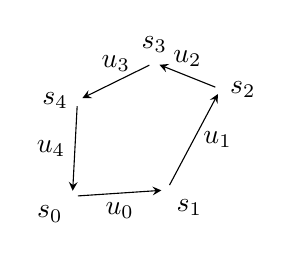
\begin{tikzpicture}[scale=.8,>=stealth]
\coordinate (a) at (0,0); \coordinate (b) at (1.5,.1); \coordinate (c) at (2.35,1.7);
\coordinate (d) at (1.3,2.12); \coordinate (e) at (.08,1.52);
\foreach \p/\q/\lbl/\pos in {a/b/0/below,b/c/1/right,c/d/2/above,d/e/3/above,e/a/4/left}
 {\draw[->,shorten <=2pt,shorten >=2pt] (\p)--(\q) node[midway,\pos] {$u_{\lbl}$};}
\foreach \p/\lbl/\pos in {a/0/below left,b/1/below right,c/2/right,d/3/above,e/4/left}
 {\node[\pos] at (\p) {$s_{\lbl}$};}
\end{tikzpicture}}

% top centre, vertex coordinates and edge coordinates
\[
\begin{aligned}
s_0&=(0,0) & u_0&=(1,0)\\
s_1&=(1,0) & u_1&=(x-1,y)\\
\big[\,\inserted{s_4=(0,f_0)}& & u_2&=(x'-x,y'-y)\\
s_2&=(x,y) & u_3&=(-x',f_0-y')\\
s_3&=(x',y') & u_4&=(0,-f_0)
\end{aligned}
\]

% upper right, seven lines
\[
\begin{aligned}
f_1&=y\\
f_2&=\underbrace{\underbrace{(\deleted{x'}x-\deleted{x}1)(y'}-y)}-y(\underline{x'}-\underline{x})\\
&=(xy'-yx')\deleted{\unsure{+}}-(y'-y)\\
f_3&=\underbrace{(x'-\underbrace{x)(f_0-y')}}+x'(\underline{y'}-\underline{y})\\
&=(xy'-yx')+f_0(x'-x)\\
f_4&=f_0x'\\
f_0&=f_0
\end{aligned}
\]

% upper middle, first brace and adjacent expression
\[
\left\{\begin{aligned}
\deleted{\unsure{y'}}y&=f_1 &&\deleted{y'=}\\
x'&=f_4/f_0\\
xy'-y'&=f_2+f_1f_4/f_0-f_1\\
xy'\deleted{\unsure{+}}-f_0x&=f_3+f_1f_4/f_0-f_4
\end{aligned}\right.
\qquad f_0x-y'=-f_1+f_2-f_3+f_4
\]

% middle, second brace and two definitions to right
{\scriptsize
\[
\left\{\begin{aligned}
y&=f_1\\
x'&=f_4/f_0\\
y'&=f_0x+{\unsure{\gamma|\chi|y|X}}_1^4
\end{aligned}\right.
\quad \gamma_1^4=f_1-f_2+f_3-f_4
\quad \gamma=f_0-f_1+f_2-f_3+f_4=\deleted{\unsure{1}}f_0-\gamma_1^4
\]
}

% middle and lower middle, substitution then quadratic
\[
\begin{aligned}
x(f_0x+\gamma_1^4)-f_0x-\gamma_1^4&=f_2+f_1f_4/f_0-f_1\\
f_0x^2+\underset{-\gamma}{\underline{(\gamma_1^4-f_0)}}x
&-(\deleted{f_1}-\deleted{f_2}+f_3-f_4+\deleted{f_2}+f_1f_4/f_0-\deleted{f_1})\\
\deleted{\unsure{x^2}}\,\cdot\, f_0x^2-\gamma x&+(f_4-f_3-f_1f_4/f_0)
\qquad \gamma=1-\gamma_1^4
\end{aligned}
\]

% lower half, root and unfinished expression
\[
x=\frac{1}{2f_0}\left(\gamma\pm\sqrt{\gamma^2-4(f_0f_4-f_0f_3-f_1f_4)}\deleted{\unsure{/f_0}}\right)
\qquad \gamma=
\]

% lower half, four-line expansion
\[
\begin{aligned}
\gamma^2={}&f_0+f_1^{\unsure{2|1}}+f_2^2+f_3^2+f_4^2-2f_0f_1+2f_0f_2
\deleted{\unsure{+}}-2f_0f_3+2f_0f_4\\
&-2f_1f_2+2f_1f_3-2f_1f_4\\
&\deleted{\unsure{+}}-2f_2f_3+2f_2f_4\\
&-2f_3f_4
\end{aligned}
\]

% bottom third, Δ, boxed pair products
\[
\begin{aligned}
\Delta={}&f_0^2+f_1^2+f_2^2+f_3^2+f_4^2-\underset{\longrightarrow}{\boxed{2f_0f_1}+\boxed{2f_0f_2}}+\boxed{2f_0f_3}-\boxed{2f_0f_4}\\
&-\boxed{2f_1f_2}+\underline{\boxed{2f_1f_3}}+2\underset{\longrightarrow}{\boxed{f_1f_4}}\\
&-\underset{\longleftarrow}{\boxed{2f_2f_3}}+\underline{\boxed{2f_2f_4}}\\
&-\boxed{2f_3f_4}
\end{aligned}
\]

% bottom third, sums at left and beneath
\[
\begin{aligned}
&=\sum f_i^2-2\sum f_i f_{i+1}+2\sum f_{i-1}f_{i+\unsure{1|2}}\\
&=\sum f_{\unsure{i|i0}}^2+2\sum f_{i+1}(f_i-f_{i-1})\\
&(f_0-f_1+f_2+f_3-f_4)^2\\
&\qquad+4(f_1f_3+f_2f_3+f_2f_4)
\end{aligned}
\]

% below bottom dividing line
\noindent\rule{\linewidth}{.3pt}
{\small
\[
u_3\wedge u_4-u_2\wedge u_3=u_3\wedge u_4+u_3\wedge u_2=u_3\wedge(u_2+u_4)
\qquad (u_4\wedge u_0)(u_3\wedge(u_2+u_4))-
\]
}

% archive sheet number: 26
